\documentclass{article}
\usepackage{amsmath}
\usepackage{amssymb}
\usepackage[top=2cm,bottom=2cm]{geometry}
\usepackage{enumerate}
\usepackage{tikz}
\usepackage{amsfonts}
\title{Homework 2}
\author{Chengyu Lin\footnote{F1003028-5100309007}}
\date{}
\begin{document}
\maketitle

\begin{itemize}
    \item[Problem 1]
        The probability of that number is a multiple of 2 is
        $1 - (\frac{1}{2})^n$.

        The probability of that number is a multiple of 5 is
        $1 - (\frac{4}{5})^n$.

        So the probability of that number is a multiple of 10 is
        $(1-(\frac{1}{2})^n) \times (1-(\frac{4}{5})^n)$.


    \item[Problem 2]

        The figure is drawn below:

    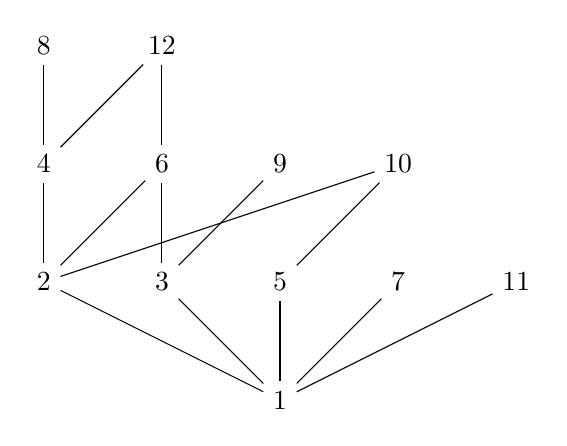
\begin{tikzpicture}[node distance=1.5cm]
        \node   (1)     {1};
        \node   (5) [above of = 1]     {5};
        \node   (3) [left of = 5]     {3};
        \node   (2) [left of = 3]    {2};
        \node   (4) [above of = 2]     {4};
        \node   (6) [above of = 3]     {6};
        \node   (7) [right of = 5]    {7};
        \node   (8) [above of = 4]    {8};
        \node   (9) [right of = 6]    {9};
        \node   (10) [right of = 9]    {10};
        \node   (11) [right of = 7]    {11};
        \node   (12) [above of = 6]    {12};
        \draw (1) -- (2);
        \draw (1) -- (3);
        \draw (1) -- (5);
        \draw (1) -- (7);
        \draw (1) -- (11);
        \draw (2) -- (4);
        \draw (2) -- (6);
        \draw (2) -- (10);
        \draw (3) -- (6);
        \draw (3) -- (9);
        \draw (4) -- (8);
        \draw (4) -- (12);
        \draw (5) -- (10);
        \draw (6) -- (12);
    \end{tikzpicture}

    \item[Problem 3]
        \begin{align*}
            (1-x)^n &= \sum_{i=0}^{n} (-1)^i x^i {n \choose i} \\
            \frac{d (1-x)^n}{dx} &=
            \sum_{i=1}^{n} (-1)^i i x^{i-1} {n \choose i}
            = -n(1-x)^{n-1}
        \end{align*}

        Simply let $x = 1$, $\sum_{i=1}^{n} (-1)^i i {n \choose i} = 0$.

    \item[Problem 4]
        Assume that $|A| = a$, $|B| = b$ and $A \cap B = \emptyset$.

        The left side of equation means that first choose $i$ elements from $A$
        and add them to $B$. Then choose $a$ elements from $B$. This is the size
        of $\{(X, Y) | X \subseteq A, |Y| = a, Y \subseteq A \cup B, X \cap Y = \emptyset\}$
        by first choosing $X$ and then choosing $Y$.

        Another way to cound the size of set above is first choosing $Y$ by
        enumerating $i = |Y \cap B|$, and then counting the number of $X$ avaiable.
        Which is $\sum_{i=0}^{a}{b \choose i} {a \choose a-i} 2^i$ and equal to the right side.

    \item[Problem 5]
        Assume that $A$ and $C$ are non-empty set.

        Denote that $a$ is the maximum of $A$ and $c$ is the minimum
        of $C$. Clearly that $c \npreceq a$.

        We have known that 

        $$\forall x, y, \sum_{x \preceq z \preceq y} \mu(x, z) = \chi_{x=y}$$
        $$\forall x, y, \sum_{x \preceq z \preceq y} \mu(z, y) = \chi_{x=y}$$

        And $X$ is a lattice so that there is a maximum 1 and a minimum 0 therefore:

        \begin{align*}
            \sum_{x \in A} \sum_{y \in C} \mu(x, y) &= -\sum_{x \in A} \sum_{y \in B} \mu(x, y) - \sum_{x \in A} \sum_{y\in A, x \preceq y} \mu(x, y) \\
            %&= -\sum_{x \in B} \sum_{y \in C} \mu(x, y) - \sum_{x \in C, x \preceq y} \sum_{y \in C} \mu(x, y)
        \end{align*}

        And for every $x \in A$, 

        $$\sum_{y \in A, x \preceq y} \mu(x, y) = \sum_{x \preceq y \preceq a} \mu(x, y) = \chi_{x = a}$$

        $$\sum_{x \in A} \sum_{y\in A, x \preceq y} \mu(x, y) = 1$$

        Now i'm going to show that 
        
        $$\sum_{x \in A} \sum_{y \in B} \mu(x, y) + \sum_{x \in B} \sum_{y \in B} \mu(x, y)
        = \sum_{x \not\in C} \sum_{y \in B} \mu(x, y) = 0$$.

        For fixed $y \in B$, 
        
        $$\sum_{x \not\in C}\mu(x, y) = \sum_{0 \preceq x \preceq y}\mu(x, y) = 0 (\text{Since }A \neq \emptyset, y\neq 0)$$

        $$\sum_{x \in A} \sum_{y \in B} \mu(x, y) + \sum_{x \in B} \sum_{y \in B} \mu(x, y) = 0$$

        Therefore $\mu(A, C) = \mu(B, B) - 1$.

\end{itemize}

\end{document}
